\documentclass[a4paper, 11pt]{article}

\usepackage{geometry}
\usepackage{layout}
\geometry{includeheadfoot, margin=3.18cm}
\usepackage{graphicx}
\usepackage{float}
\usepackage{array,booktabs}
\usepackage[style=numeric,sorting=debug,backend=biber]{biblatex}
\usepackage[T1]{fontenc}
\usepackage{todonotes}
\usepackage{paralist}
\usepackage{listings}
\usepackage{lmodern}
\usepackage{minted}
\usepackage[fleqn]{amsmath}
\usepackage{hyperref}
\usepackage[center]{caption}
\hypersetup{
  colorlinks,
  citecolor=black,
  filecolor=black,
  linkcolor=black,
  urlcolor=black
}
\usemintedstyle{autumn}
\lstset{language=SQL}
\addbibresource{report.bib}
\DeclareDatamodelEntrytypes{standard}
\DeclareDatamodelEntryfields[standard]{type,number}
\DeclareBibliographyDriver{standard}{%
  \usebibmacro{bibindex}%
  \usebibmacro{begentry}%
  \usebibmacro{author}%
  \setunit{\labelnamepunct}\newblock
  \usebibmacro{title}%
  \newunit\newblock
  \printfield{number}%
  \setunit{\addspace}\newblock
  \printfield[parens]{type}%
  \newunit\newblock
  \usebibmacro{location+date}%
  \newunit\newblock
  \iftoggle{bbx:url}
    {\usebibmacro{url+urldate}}
    {}%
  \newunit\newblock
  \usebibmacro{addendum+pubstate}%
  \setunit{\bibpagerefpunct}\newblock
  \usebibmacro{pageref}%
  \newunit\newblock
  \usebibmacro{related}%
  \usebibmacro{finentry}}
% Stop Latex from repositioning tables like an idiot
\restylefloat{table}

\begin{document}

\begin{titlepage}

\newcommand{\HRule}{\rule{\linewidth}{0.5mm}} % Defines a new command for the
% horizontal lines, change thickness here

\center

\textsc{\LARGE Imperial College London}\\[1.5cm]
\textsc{\Large Department of Computing}\\[0.5cm]
\textsc{\large 3rd Year Group Project Report}\\[0.5cm]

\HRule \\[0.4cm]
{\huge \bfseries Translation of}\\[0.4cm]
{\huge \bfseries First Order Predicate Logic to SQL}\\[0.4cm]% Title of your document
\HRule \\[1.5cm]

\begin{minipage}[t]{0.4\textwidth}
  \begin{flushleft} \large
    \emph{Authors:}\\
    Sean \textsc{Allan}\\
    Mitchell \textsc{Allison}\\
    Sam \textsc{Esgate}\\
    Thomas \textsc{Harling}\\
    Ted \textsc{Sales}\\
    Max \textsc{Tottenham}
  \end{flushleft}
\end{minipage}%
%
\begin{minipage}[t]{0.4\textwidth}
  \begin{flushright} \large
    \emph{Supervisor:} \\
    Dr. Fariba \textsc{Sadri}  % Supervisor's Name
  \end{flushright}
\end{minipage}%
\\[4cm]

{\large \today}\\[3cm] % Date, change the \today to a set date if you want to be precise

\vfill % Fill the rest of the page with whitespace

\end{titlepage}

\renewcommand{\contentsname}{\huge Contents \vspace{1cm}}
\tableofcontents
\clearpage

\setlength{\parskip}{0.3cm} \setlength{\parindent}{0cm}

\section{Executive Summary}
  At its heart our project is a language translator, taking as input a
  restricted version of first-order predicate logic, and producing as output
  the corresponding SQL, for a given domain. This allows any SQL relational
  database to be queried using only first-order predicate logic, without the
  user needing to know any SQL. The implications of this open up
  new avenues in the realms of teaching and computer security, or
  alternatively integration as a component of a larger system.

  The predominant use-case for our project would be as a teaching tool,
  suitable for use by students studying both logic and databases, topics which
  many universities deem to be mandatory for all computing students. To
  reinforce a students understanding of logic, queries can be written and tested
  against a suitably populated database of facts. The result of these queries
  can then be used to determine how well they have understood the course
  material.

  The generated SQL could be used as a reference for the student, either to
  highlight issues with their logic or to explain the formulation of correct
  SQL, providing them with extensive revision notes.

  The project also lends itself to creating problem sheets for these subjects.
  For example, a teacher could create a list of questions in english, like
  ``what are the names of dragons that are happy?'' requiring the student to
  give both the predicate logic and the SQL yielding the answer to that
  question. Our project could then be used to easily check the student's work.

  \todo[inline]{Too much stuff on the security... A wild Farfetch'd appears!}

  Conversely, in the world of computer security access to data is an important
  topic, and one which has come to public attention through the recent leaks
  from former NSA employee Edward Snowden.

  Imagine a scenario where a company needs to work with another large
  organisation, for example a telecoms firm working with the US Government. The
  company respects customer privacy rights, and so wants to give the government
  as little customer information as possible, whilst still allowing them to do
  their job. This is known as the principle of least privilege.

  Our project provides the bedrock for such a security system, which
  abstracts away from any database where customer data is stored, allowing
  questions to be asked (in predicate logic) by the government and answered in
  the most desirable manner with respect to the company's privacy policy.

  Finally, there is scope for integrating this project with a larger system
  whose goal is, for example, to create business analytics using only an
  English description of the required information. If such a system had a
  method of converting English into predicate logic, it would be trivial to
  give this to our project to allow the larger system to give actual database
  analytics answers for the English description.

  \subsection*{Elevator Pitch (quite a hard sell)}
  \todo[inline]{I swear this is the same thing as the executive summary?}
  In summary, we have created a system that creates SQL queries from logic 
  statements. This allows you to query a database without knowing anything
  about SQL and importantly to ignore which variant of SQL you
  are using and get on with extracting data. It provides the basis for a
  unique teaching tool for both SQL and logic and it brings some power
  of logic to regular databases, without the need to migrate to datalog.

  What is your Project? What does it do? Why would I want to buy it? etc.
  No implementation, software engineering details, or project management

\section{Introduction}

  Set the scene ... motivation'
  State the problem you are trying to solve ...objective(s)
  Summarise your main achievements 

When we began this project our goal was simply to allow a database to be 
queried using logic. You shouldn't need to know the syntax of a particular
version of SQL, you shouldn't have to explicitly tell the DBMS how to extract
the data, all you need to do is write a query in logic and we will
get it for you.

We wanted to make it as easy as possible to write queries and view results;
our objective was to make it easy to understand, easy to write and to
provide clear advice when it does go wrong.

At the end of the project we can say that we have achieved most of our initial 
goals. We have created a system that can convert the queries, we have created
a simple way to construct and edit these queries, one that can be changed to 
work on any database and will provide clear error messages.

  -- GOALS - In Chatley coursework 1 --
  Unfortunately there aren't any goals in the chatley coursework one.
  Just a bunch of questions, turns out we forgot to add them. WHOPS LOOL
  TODO: Discuss goals, they're referenced in the Project Management
  section. Revisions should not be talked about here though, just the
  overarching goals of the project.

\section{Background Research}
\label{sec:background}
\subsection{SQL}
  Structured Query Language (SQL)~\cite{wiki:SQL} is a special-purpose
  programming language designed for managing data held in relational database
  management system. SQL is made up of two different types of language:

  \begin{itemize}
      \item
        Data Definition Language. DDL is used to define the structure of a
        database (also known as its schema).
      \item
        Data Manipulation Language. DML is primarily used to insert, select,
        delete and update data within a database.
  \end{itemize}

  However, as defined by the SQL92 standard\cite{isoSQL}, read-only operations
  such as 'SELECT' (without 'INSERT INTO') should not exist as part of the DML;
  they do not manipulate the data, only query it. This distinction between
  read-only and read-write operations is not enforced, but here we will focus
  only on read-only operations (so called 'SQL-data' operations).

\subsection{Tuple Relational Calculus}
  SQL was originally based on Relational Algebra and Tuple Relational
  Calculus. RA forms the structure and operations that can be performed
  across tuples of data and TRC provides a query language for such a model.

  \subsubsection{Formal Specification of Tuple Relational Calculus\cite{lecRA}}
    \label{sec:formalTRC}
    A query takes the form: \{T | p(T)\}

    The answer is the set of all tuples T such that p(T) evaluates to true.

    A formula F is recursively defined as:
    \begin{itemize}
      \item $p(t_1, ..., t_n)$ where predicate $p$ is applied to terms $t_1, ..., t_n$ (atomic formula)
        \item $\lnot F$ where $F$ is a formula.
        \item $F' \land F''$ where $F', F''$ are formulae.
        \item $F' \lor F''$ where $F', F''$ are formulae.
        \item $\exists t(F)$ where $F$ is a formula and $t$ is a tuple of terms.
        \item $\forall t(F)$ where $F$ is a formula and $t$ is a tuple of terms.
      \end{itemize}

      $\exists t(F)$ is true if, for some tuple $t$ the formula $F$ is true. \\
      $\forall t(F)$ is true if, for all tuples $t$ the formula $F$ is true.

      A variable $v$ is bound in $F$ if it is of the form:

      $\exists t(F)$ or $\forall t(F)$ and $v \in t$.

      Otherwise $v$ is said to be free.
      
      Note that in query \{T | p(T)\} the variables in T must be the only
      free variables in p(T).

    \subsubsection{Querying Relational Algebra}
      Using all of this, it is possible to begin formulating some simple
      queries. For example, suppose it was desirable to query all films from a
      particular director in a database. It would be simple to write:

      \begin{center}
        \{F | F $\in$ Films $\land$ F.director = "Matt Damon"\}
      \end{center}

      This would however return all the elements of the tuple. The tuple may
      contain many irrelevant values to the user, and so it would be desirable
      to only return the title of said film. This could be achieved as detailed
      below:

      \begin{center}
        \{F | $\exists$F1 $\in$ Films(F1.director = "Matt Damon" $\land$ 
          F.title = F1.title)\}
      
        \emph{NOTE: F becomes a tuple with one element called title.}
      \end{center}

      We are now able to represent projection and selection. We can also
      represent joins. Let us suppose that we wish to find all titles of films
      whose director has also directed another film.

      \begin{center}
        \{F | $\exists$F1 $\in$ Films($\exists$F2 $\in$ 
        Films(F1.director = F2.director $\land$ F1 != F2)
        \\ $\land$ F.title = F1.title)\}
      \end{center}

\subsection{Mapping Tuple Relational Calculus to First-order Predicate Logic}
    With the knowledge of TRC, and how it underpins SQL, it is now necessary to
    formulate a mapping between TRC and first order predicate logic.

    \subsubsection{Atoms, Formulae, Predicates}
      Firstly atoms, formulae and predicates remain unchanged. We still wish to
      find a set of tuples that will result in a given formula evaluating to
      true.

    \subsubsection{Set Membership}
      Whereas before we could simply test the membership of a tuple $t$ in a
      relation $R$ with $t \in R$, first order predicate logic does not have
      the notion of set membership. From here there are a few different
      solutions to the problem.

      One solution is with an 'InRelation' predicate, where 'InRelation(t, R)'
      would have the same semantic meaning as the previous set membership test.
      This seems to work, although throughout first order predicate logic, we
      do not have the notion of a tuple; an atom is structurally meaningless. A
      disadvantage of this would be that accessing members of the tuple would
      require another predicate, for example 'InTuple(a, 'attrName', t)' which
      would have the same semantic meaning as 't.a' in TRC.

      Another solution, which solves the previous issue, is to generate n-ary
      predicates that represent a tuple. For example, given a relation 'films',
      with columns 'title', 'length' and 'date-released', a predicate
      'films(title, length, date-released)' could be generated, where title,
      length and date-released are all variables. This certainly solves the
      issue the set membership issue, but does add uneccessary bloat to each
      query; relations may have thousands of columns, very few of which are
      likely needed in a given query.

      The solution chosen addresses the issues raised so far.

      For a relation R(k, $a_{1}$, $a_{2}$, ..., $a_{n}$) with primary key k
      and n attributes we generate n + 1 predicates:
      \begin{align*}
        \text{1:  }     & R(k)            \\
        \text{2:  }     & R.a_1(k, a1)   \\
        \text{3:  }     & R.a_2(k, a2)   \\
                        & \vdots          \\
        \text{n + 1:  }  & R.a_n(k, an)
      \end{align*}

      Relating a tuple to its primary key gives a concise way to address it,
      adding the slight restriction that each relation must have a primary key.

    \subsubsection{Free and Bound Variables}
    \label{sec:freebound}

      Looking back to Tuple Relational Calculus in
      section~\ref{sec:formalTRC}, we will use similar semantics for free and
      bound variables. Recall the syntax for the return value in TRC, $T$ in the
      query below

      \{T | p(T)\}

      That is to say that TRC returns the set of all tuples $T$, such that 
      $p(T) \models \top$. Without extending predicate logic, we cannot use 
      a similar format for specifying what is returned. However, all 
      variables that are free in $p(T)$ must be in $T$ and so we assume 
      that all unbound variables in the query are to be returned.

  \section{Translation of First-order Predicate Logic to SQL}

    Section~\ref{sec:background} provides a rough translation between
    first-order predicate logic and tuple relational calculus, and from this
    grounding we can begin to define the mapping between logic and SQL.
    First-order predicate logic is more expressive than SQL,
    \todo[inline]{Back this up. I believe it is true but how can it be proved?}
    \todo[inline]{
      Sam. I'm not sure this is true.
    
      Codd's Theorem: Relational Calculus is as expressive as Relational Algebra.

      Word on the Street: Relational Calculus is equivalent to First-Order Logic.
    
      Therefore First-Order Logic is as expressive as Relational Algebra.

      SQL is built on Relational Algebra (adds grouping, aggregation, arithmetic). 
      
      Therefore it makes sense that SQL is at least as expressive as First-Order Logic, if not more?

      Slightly out of my depth here, but intuitively it kind of makes sense - can you get the size of a set in logic? No. Can you in SQL? Yes.

      There were SQL features that we had no idea how to represent in pure logic, we found ourselves wanting to create special syntax for them (because logic cannot describe count, sum etc.)
    }

    and so there will not always exist a
    translation between logic and SQL. For this reason, this section will aim
    to describe common SQL queries or patterns in terms of their logical
    equivalence.

    The examples in the section below will make use of the filmdb as used in
    the project. A description of the SQL schema can be found in the appendix.

    \subsection{SQL SELECT}

    The SELECT statement is used to select data from a database.\cite{w3SELECT}
    Suppose that we wish to query the database for every film title in the
    database. Below is an example of an SQL query that satisfies this criteria.

    \begin{minted}{sql}

    SELECT title
    FROM films;

    \end{minted}

    This is equivalent to the following first-order predicate logic query.
    \begin{gather}
      \exists x(films.title(x, title)) \label{select1}
    \end{gather}
    The query binds $x$ and leaves $title$ free, meaning that our
    answer will be the set of all subtitutions for $title$ such that
    $\exists x(films.title(x, title)) \models \top$. The '$\exists$' symbol
    serves two purposes. Firstly it binds $x$ as mentioned above, and secondly
    it enforces that the substituted $title$ exists in at least one tuple.
    The predicate $films.title$ gives the translator the scope of
    relations to query (in this case, just the $films$ relation).

    Strictly speaking since tuple relational calculus is based on set
    operators, like relational algebra, and SQL implcitly uses bag operators
    this actually evaluates to the following:

    \begin{minted}{sql}

    SELECT DISTINCT title
    FROM films;

    \end{minted}

    Note that it is perfectly valid to create a query with no bound variables,
    such as:
    \begin{gather}
      films.title(x, title) \label{select2}
    \end{gather}
    This will return the set of all tuples of the form \{$films.fid,
    films.title$\}, using the following SQL query.

    \begin{minted}{sql}

    SELECT fid, title,
    FROM films;

    \end{minted}

    Note that the DISTINCT keyword is no longer needed, as $films.fid$ is a
    primary key.

    Now we have demonstrated projecting a primary key, and a single attribute,
    all that is left is to project multiple attributes from a tuple. This
    requires the conjunction of multiple predicates, each over the same
    relation and using the same primary key (that is to say that each predicate
    relates to a single tuple). Suppose we wish to project
    every film title, and its corresponding length.

    \begin{gather}
      \exists x(films.title(x, y) \land films.length(x, z)
    \end{gather}

    As both $y$ and $z$ are from the same unique tuple identified by $x$
    (enforced by the conjunction within the query) our
    answer is equivalent to that returned by the following SQL query.

    \begin{minted}{sql}
    SELECT name, length
    FROM films;
    \end{minted}

    This can be extended to any number of predicates, although the relation and
    the key must be the same. If this is not the case, the query may represent
    a join, later described in section~\ref{sec:joins}.

  \subsection{SQL WHERE}

    The WHERE clause is used to extract only those records that fulfill a
    specified criterion.~\cite{w3WHERE} 

    \subsubsection{Equality}

      Suppose that we wish to check the existence of a film (The Bourne
      Identity) within our database. Below is an SQL query that satisfies this
      criteria.

      \begin{minted}{sql}

      SELECT title,
      FROM films
      WHERE title = 'The Bourne Identity';

      \end{minted}

      We expect to encounter at least one tuple if the film exists in our domain
      of discourse. \todo{Cite this from our AD lectures} This can be represented
      in one of two ways in first-order predicate logic.
      \begin{gather}
        \exists x(films.title(x, y) \land y = \text{'The Bourne
        Identity'})\label{where1}\\
        films.title(x, \text{'The Bourne Identity'})\label{where2}
      \end{gather}
      Both of these queries are valid, however note that they do return different
      tuples. (\ref{where1}) returns the same answer as the SQL query above, although
      it is verbose. (\ref{where2}) returns the singleton tuple \{$films.fid$\},
      because under our definition, only free variables are returned. Most of
      the time this is acceptable, as it is often undesirable to return a
      constant term in the results, and also has the benefit of being more
      compact.

      So far we have used the notion of equality to bind variables to specific
      ground terms. We can also use equality to ensure that two variables have
      the same value. For example, consider the following logical query.
      \begin{gather}
        \exists a,b,y(actor.name(a, x) \land film.director(b, y) \land x = b)
      \end{gather}
      The query returns names of all of the actors who have also directed a
      film. This translates to the following SQL query. For now, do not dwell
      on the cross join, as this will be explained in further detail in
      section~\ref{sec:joins}.

      \begin{minted}{sql}
      SELECT name
      FROM actors CROSS JOIN film
      WHERE name = director;
      \end{minted}

      Note, that it is also possible to write the logic query in a more succint
      manner, as follows.
      \begin{gather}
        \exists a,b(actor.name(a, name) \land film.director(b, name))
      \end{gather}
      Here we have removed the equality constraint, instead unifying both
      predicates to the same variable. This is often a more desirable way to
      specify logical queries.

    \subsubsection{Inequality}

      Suppose that we wish to check the inverse of the previous section, that
      there exists other films except 'The Bourne Identity'. In SQL, this
      simply translates to the following.

      \begin{minted}{sql}
        SELECT title,
        FROM films
        WHERE title <> 'The Bourne Identity';
      \end{minted}

      The existence of one or more tuples satisfies our query; if no queries
      are returned, it must be the case that there are no other films except
      'The Bourne Identity'.

      As before, there are two ways we can represent the SQL query above in
      logic.
      \begin{gather}
        \exists x(films.title(x, y) \land y !=  \text{'The Bourne
        Identity'})\label{where3}\\
        \lnot films.title(x, \text{'The Bourne Identity'})\label{where4}
      \end{gather}
      The first query matches the output of our equivalent SQL query, but again
      is more verbose. The second returns the set of singleton tuples
      \{$films.fid$\} such that the title associated with that particular
      primary key is not 'The Bourne Identity'. This is not equivalent to our
      SQL expression however, and may be undesirable to use in this
      circumstance (it is likely that we would like to return all other film
      titles).

      \todo{Do we use <= or $\le$}

      We can also express other inequalities, such as '<', '<=', '>', '>='.
      Here we query for all the fid of every films with length greater than or
      equal to two hours.

      \begin{minted}{sql}
      SELECT fid,
      FROM films,
      WHERE length >= '2:00:00';
      \end{minted}

      This can be expressed using the following predicate logic query.
      \begin{gather}
        \exists x(films.length(x, y) \land x >= \text{'2:00:00'}) \label{where5}
      \end{gather}

      Queries can be constructed for the other inequalities in a
      similar manner.

    \subsubsection{Logical Connectives}

      It is often desirable to project a set of attributes from a statement
      made up of conditions and logical connectives. For example, suppose we
      wished to query the database for all film titles where the film is between 
      two and three hours in length. The relevant SQL query would take one of
      the following forms.

      \begin{minted}{sql}
      SELECT title
      FROM films
      WHERE films.length >= '2:00:00'
        AND films.length <= '3:00:00';

      SELECT title
      FROM films
      WHERE films.length BETWEEN '2:00:00' AND '3:00:00';
      \end{minted}

      This can simply be represented in first-order predicate logic with the
      following query.

      \begin{gather}
        \exists x, length(films.title(x, title) \land films.length(x,
        length)\\
        \land length >= '2:00:00' \land length <= '3:00:00')
      \end{gather}

      Notice how the last two constraints in the logical query translate
      with very little effort. The same applies to constraints seperated with
      an $\lor$ which is equivalent to OR in SQL.

  \subsection{Joins}
    \label{sec:joins}

    An SQL JOIN clause is used to combine rows from two or more tables, based
    on a common field between them.~\cite{w3JOINS} Joins can enable incredibly
    powerful queries, especially where information
    is normalized (split across many relations) to minimise duplication.

    \subsubsection{SQL CROSS JOIN}

      A cross join is equivalent to the cartesian product of two sets. Suppose
      that we wished to write a query that returned every possible pair of
      film title and actor name in the database. In ANSI-89 SQL, we could use 
      the following query.

      \begin{minted}{sql}
      SELECT title, name
      FROM films, actors;
      \end{minted}

      Alternatively, in ANSI-92 SQL we can explicitly write:

      \begin{minted}{sql}
      SELECT title, name
      FROM films CROSS JOIN actors;
      \end{minted}

      We can think of this query as the conjunction of two disjoint relations;
      the relations do not share a key, or if they do we are not using them as
      part of the join.

      \begin{gather}
        \exists fid, aid(films.title(fid, title) \land actors.name(aid, name))
      \end{gather}

      The example used is unlikely to be a useful query on the database. Cross
      joins are rarely used in this format. Instead, they are often combined
      with a WHERE clause to extract useful information. For example, if we
      wished to query every actor that acted in the film 'The Bourne Identity',
      we could could use the following logic query.

      \begin{gather}
        \exists fid(films.title(fid, \text{'The Bourne Identity'}) \nonumber\\
        \land actors.fid(aid, fid) \land actors.name(aid, name))
      \end{gather}

      Which specifies that we only wish to return the set of all singleton
      tuples \{$name$\} such that the actor starred in 'The Bourne Identity'.
      With our knowledge of SQL CROSS JOIN, we can express this as the
      following SQL query.

      \begin{minted}{sql}
      SELECT name
      FROM films CROSS JOIN actors
      WHERE films.fid = actors.fid AND films.title = 'The Bourne Identity';
      \end{minted}

      So far we have not discussed SQL aliases. Aliases are required if joining
      two instances of the same relation. To demonstrate this, suppose that we
      wish to generate the set of all pairs of actors that have appeared in the
      same film. This is achieved with the following SQL query.

      \begin{minted}{sql}
      SELECT a1.name,
             a2.name
      FROM films CROSS JOIN actors AS a1
        CROSS JOIN actors AS a2
      WHERE films.fid = a1.fid AND films.fid = a2.fid 
        AND a1.name != a2.name
      \end{minted}

      Notice that we cannot simply refer to the relation $actors$ anymore, as
      there are two of them; without an alias, the identifier would be
      ambiguous. Below is a representation of the query in logic.

      \begin{align}
          \exists fid, & a1, a2(  \nonumber\\
                       & films(fid) \land \nonumber\\
                       & actors.fid(a1, fid) \land actors.fid(a2, fid) \land \nonumber\\
                       & actors.name(a1, name1) \land actors.name(a2, name2) \land \nonumber\\
                       & name1 != name2 \nonumber\\
        ) \hspace{6mm} &  % Ignore horrendous bodge...
        \label{largeCROSS}
      \end{align}

      \todo{Actor doesn't have an fid field. Did we do this so we wouldn't have to mess about with casting?}

    \subsubsection{SQL INNER JOIN}

      Introduced in ANSI-92 SQL, INNER JOIN allows for a more readable version of
      the above CROSS JOIN, WHERE combination. The logical query~\ref{largeCROSS}
      can be written using the SQL INNER JOIN syntax as:

      \begin{minted}{sql}
      SELECT a1.name,
             a2.name
      FROM films CROSS JOIN actors AS a1
        CROSS JOIN actors AS a2
      ON films.fid = a1.fid AND films.fid = a2.fid 
        AND a1.name != a2.name
      \end{minted}

      INNER JOIN is the same as JOIN as of ANSI-92 SQL, and it the existence of
      the ON clause is not necessary (making it a cross join).

    \subsubsection{Translating to the Correct Join}

      Fundamentally, joining two relations often occurs as the result of a
      conjunction of predicates when translating from first-order predicate
      logic. However, there are a few different circumstances which affect the
      type of join that must be used. Figure~\ref{fig:jointranslation} explains
      the different types of join that can result from a query.

      \begin{table}
        \label{fig:jointranslation}
        \begin{tabular}{ | p{\dimexpr 0.22\linewidth-2\tabcolsep} |
          p{\dimexpr 0.22\linewidth-2\tabcolsep} |
          p{\dimexpr 0.15\linewidth-2\tabcolsep} |
          p{\dimexpr 0.41\linewidth-2\tabcolsep} | } \hline
        LHS & RHS & Join & Explanation \\
        \hline
        $rel.attr1(k, a)$ & $rel.attr2(k, b)$ & No Join & 
        Both keys and relations are equal. This conjunction involves projecting
        two elements from the same tuple, and so no join is necessary.\\ \hline
        $rel1.attr1(k1, a)$ & $rel2.attr2(k2, b)$ & CROSS JOIN &
        The keys are different and the relations may or may not be equal. Here
        we assume that a != b. As there are no common elements, a cross join
        must occur.\\ \hline
        $rel1.attr1(k1, a)$ & $rel2.attr2(k2, a)$ & JOIN ON rel1.attr1 =
        rel2.attr2 &
        The keys are different, but the attributes rel1.attr1 and rel2.attr2
        are equal, thus we must join on these elements. Note that aliases are
        used to avoid ambiguity between the two sets of attributes if they
        overlap. Note that this may be combined with the example below to
        create a more complex join.\\ \hline
        $rel1.attr1(k, a)$ & $rel2.attr2(k, b)$ & JOIN ON rel1.key =
        rel2.key &
        The keys are the same and we assume the attributes rel1.attr1 and rel2.attr2
        are different. We must join on the keys. Note that aliases are
        used to avoid ambiguity between the two sets of attributes if they
        overlap. Note that this may be combined with the above example to
        create a more complex join.\\ \hline
      \end{tabular}
        \caption{A table explaining the correct join to use for a logical query
        conjunction.}
    \end{table}


  \subsection{SQL EXISTS}
    The SQL EXISTS condition is used in a SQL query and is considered "to be
    met" if the subquery returns at least one row.\cite{technetEXISTS} The
    condition is useful in translating predicate logic to SQL, as it's meaning
    is consistent across both languages. 

    \subsubsection{Existentially Quantifier Variables}
    \label{sec:existential}
    Often in a logical query, it will be common to existentially quantify a
    variable in an inner subquery. For example, the following subquery checks
    the existence of any films within our database with the same name, but that
    are not the same film, and returns the name of said film.
    \begin{multline}
      \exists title(films.title(x, title) \land \exists title(films.title(y,
      title) \land x != y))
    \end{multline}
    With a query of this format, we can simply translate the subquery, wrap it
    in an SQL EXISTS condition and conjunct this onto the WHERE clause of the
    outer query's query.

    \begin{minted}{sql}
      SELECT films1.title
      FROM films AS films1
      WHERE EXISTS (
        SELECT films2.title
        FROM films
        WHERE films1.fid <> films2.fid );
    \end{minted}

    There are two things to note with this approach, both relating to scope.
    The first is that the tables should be aliased. SQL requests that aliases
    for inner subqueries must not have been used previously; the outer scope is
    available to the inner subquery. The second is that, although we have not
    specified that films2.fid is not to be returned, it cannot be. The outer
    SELECT is not in the same scope as the inner SELECT, and so we must create
    an exception to the free and bound variable rules that we specify in
    section~\ref{sec:freebound}.

    We could also repesent the previous query in a simpler form.
    \begin{multline}
      \exists x,y(films.title(x, title) \land films.title(y, title)
        \land x != y)
    \end{multline}
    Which would translate to the following SQL query.

    \begin{minted}{sql}
    SELECT films1.title
    FROM films as films1 JOIN films as films2 ON films1.title = films2.title
    WHERE films1.fid <> films2.fid;
    \end{minted}

    Each of these forms are equivalent, and will return the same result.
    However, it is useful to be able to represent nested quantifiers, as it
    will not always be equivalent to combine them.\cite{washEQUIV}

    \subsubsection{Universally Quantified Variables}
    Using our knowledge from section~\ref{sec:existential}, we can now
    formulate a translation for universally quantified variables. In
    first-order predicate logic, the following equivalence holds:
    \begin{multline}
      \forall x(P(x)) \equiv \lnot \exists x(\lnot P(x))
    \end{multline}
    We can use this equivalence to simply encounter universally quantified
    variables as existentially quantified. Below is an example query in logic
    that aims to return all directors such that every film that they have
    directed is longer than one hour.
    \begin{multline}
      \exists x(films.director(x, director) \land \forall y(films.director(y,
      director) \land films.length(y, length) \land length > '1:00:00'))
    \end{multline}
    We can think of this equivalently as following.
    \begin{multline}
      \label{eqn:except}
      \exists x(films.director(x, director) \land \lnot \exists y,length(\lnot(films.director(y,
      director) \land films.length(y, length) \land length > '1:00:00')))
    \end{multline}

    Using De Morgan's laws, we can infer the following
    equivalence.
    \begin{multline}
      \label{eqn:demorganequiv}
      \lnot(films.director(y, director) \land films.length(y, length) 
      \land length > '1:00:00') \equiv (films.director(y,
      director) \lor films.length(y, length) \lor length > '1:00:00')
    \end{multline}
    Equation~\ref{eqn:demorganequiv} however does not offer much progress, as
    we have not yet specified how to evaluate disjunction.

    Instead we must look to the query's semantic meaning. Referring to
    section~\ref{sec:except}, it can be seen that we need to make use of the
    SQL EXCEPT operator.

    Our logical query now can be translated to the following SQL query.
    \begin{minted}{sql}
    SELECT film1.director
    FROM films AS films1
    WHERE NOT EXISTS (
      SELECT films2.director
      FROM films AS films2
      EXCEPT
      SELECT films2.director
      FROM films AS films2
      WHERE films2.length > '1:00:00' AND films2.director = films1.director);
    \end{minted}

  \subsection{SQL EXCEPT}
    The SQL EXCEPT operator takes the distinct rows of one query and returns
    the rows that do not appear in a second result set.\cite{wiki:EXCEPT}

    As seen in the previous example, it may be the case that we need to negate
    a set of predicates.By example, we will refer to the subquery within
    equation~\ref{eqn:except}:
    \begin{multline}
    \exists y(\lnot(films.director(y,
      director) \land films.length(y, length) \land length > '1:00:00'))
    \end{multline}
    Semantically, we wish to prove that a y exists, such that y is the films
    fid, and the length of that film is above one hour. We could formulate the
    translation as below:
    \begin{minted}{sql}
    SELECT films.director
    FROM films
    WHERE length <= '1:00:00';
    \end{minted}
    So the answer is simply achieved by negating the condition. However, if
    there are other constraints in the query that create a join, we do not wish
    to negate these; we only wish to negate the conditions that restrict the
    data after a join. The simplest method here to solve this problem is to use
    the EXCEPT operator. The above SQL query is equivalent to the following.
    \begin{minted}{sql}
    SELECT films.director
    FROM films
    EXCEPT
    SELECT films.director
    FROM films
    WHERE length > '1:00:00';
    \end{minted}

  \subsection{NULL Values}

      \todo[inline]{I imagine here would be a good place to talk about NULLs.
      Max, we should go over our specification for NULL.}

\section{Design and Implementation}
  Anandha: Summarise key implementation details (how did you do it? what technology was
  used

  \todo{and why? what other technology was considered, but not used and why? Any technical challenges encountered and how addressed?  Any risks anticipated, and how mitigated.}

  It was decided that the project would be written in Python. This was due to
  the large number of plugins and frameworks available. Also since Python is
  interpreted there would be no large compile time which would speed up the rate
  of work.

  The decision was taken to create a website and not a standalone application.
  Doing so would ensure that users would always be using the most up to date
  code, since all of the logic to SQL conversion would be handled on the server
  and not on their own machines. (add more reasons if you can think of them...
  was making the GUI nice easier?)


  \todo[inline]{ List of Packages Used:\\

                 Backend\\
                 -------\\
                 psycopg2   - Database Connection\\
                 PLY        - Parser Generator\\
                 Config Parser - parsing configuration files\\

                 Middleware\\
                 ----------\\
                 RabbitMQ   - Message Broker (acts as a task queue)\\
                 Celery     - Sets up a worker to pull jobs off task Q\\
                 Web.py     - Web Server\\

                 Front End\\
                 ---------\\
                 ACE        - Text Editor\\
                 jQuery     - ubiquitous JS library\\

                 Testing\\
                 -------\\
                 nose       - Testing Framework\\
                 paste      - Test utilities for generating web requests\\}

  \subsection{Front-end site}
    \subsubsection{Web server}
      The web.py framework (link to http://webpy.org/ ) was chosen to host the
      user facing site. Doing so allowed us to quickly set up a functioning site
      and concentrate on developing useful features, instead of spending a large
      amount of time setting up a more complicated web server.

      The JSON data format was used to transfer the logic input by the user to the
      server and the translated SQL to the user from the server. The format was
      chosen as it was very easy to parse by Javascript running in the user's
      browser and was well documented online due to its wide existing use.

    \subsubsection{Webpage plugins and libraries}
      The site made heavy use of jQuery, which greatly simplified the handling
      of JSON data sent between the user and the server.

    \subsubsection{Graphical user interface}
      \begin{figure}[h!]
        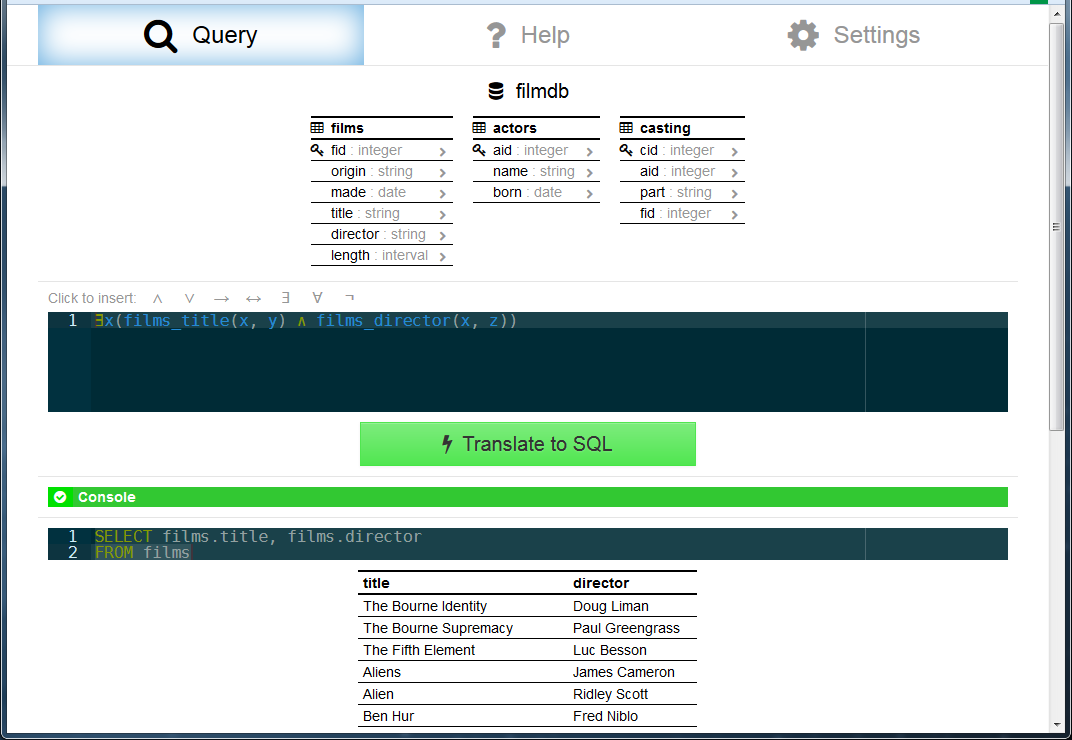
\includegraphics[width=\textwidth]{images/Site.png}
        \caption{Web App Main Page}
      \end{figure}

      The interface that the user would see and interact with had to be simple
      and intuitive to use. In particular, this meant that logic queries had to
      be easy to input and the resulting SQL and the result of running it on the
      database had to be easy to read and understand.

      The javascript Ace http://ace.c9.io code editor was used for inputting the
      user's logic query. The editor was both extremely powerful and very easy
      to implement. The editor provided a familiar interface when compared with
      desktop applications such as Vim or Gedit.

      The editor had a number of advantages over using a simple text box form.
      This included syntax highlighting, line numbers, displaying hidden
      characters and providing many different themes.

      Syntax highlighting was achieved by (Ted magic). Syntax that the
      highlighting was able to distinguish between included logic symbols,
      brackets, data types.

      \begin{figure}[h!]
        \centering
        
\includegraphics[]{images/LogicSymbols.png}
        \caption{Buttons to insert logic symbols}
      \end{figure}

      Logic symbols could be input both with key shortcuts and with dedicated
      buttons. For instance, the AND symbol could be input by typing
      forwardslash then backslash. This ensured that it was easy for new users
      to start using the web app (using the provided buttons), whilst also
      allowing experienced users to quickly input larger queries (using key
      shortcuts).

      \begin{figure}[h!]
        \centering
        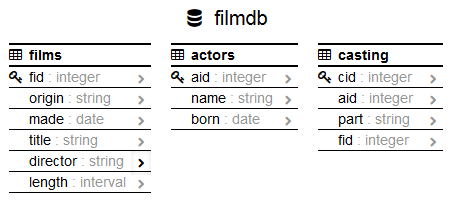
\includegraphics[]{images/Schema.png}
        \caption{Database name, tables and table schemas displayed}
      \end{figure}

      Information about the database schema was prominently displayed at the top
      of the main page. The data included the database name, table names, table
      attributes, attribute types and marking of the primary key. Without this
      information the user could easily forget the exact names of each attribute
      that they wanted to use, or not know the correct datatype to use in their
      logic query.

      \begin{figure}[h!]
        \centering
        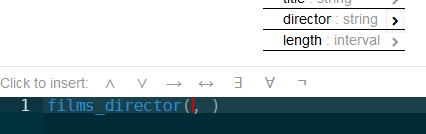
\includegraphics[]{images/InsertLogic.png}
        \caption{The arrow next to 'director' inserts the relevant logic}
      \end{figure}

      To further simplify and increase the speed of writing logic queries,
      each table attribute had an arrow button placed next to it. When clicked,
      the button would insert the appropriate logic syntax into the logic query
      field. This feature helped to significantly reduce the number of syntax
      errors caused by small spelling mistakes, and helped the user to input
      correct logic syntax.

      The site was designed with the fewest number of pages possible, in order
      to maintain its simplicity and ease of use. When a user browses to the
      site, the homepage is the logic translation page. This allows the user to
      begin working straight away, with no setup costs or many pages to first
      browse through.

      In addition to the translation page, there is also a help page and a
      database setup page. The help page provides an easy to understand guide
      on how to write and form logic queries, whilst the database setup page
      allows the user to specify their own database to connect to and run
      queries on. The links to these two pages are placed at the top of the page
      so that they are easily accessible.
 
      Picked nice colours and text styles.

  \subsection{Middleware plugins}
    \subsubsection{Celery and RabbitMQ}
      By default web.py is multithreaded, meaning that each users request is
      handled in a separate thread, this allows multiple users to sent http
      requests to the server at once. Because of this, it would indeed be
      possible to run the translation code in the same thread that services 
      a users web-request. However in an effort to make our project scalable we
      decided to use a 3 tiered architecture. The web server dispatches a job to
      RabbitMQ, a Celery worker listens to the RabbitMQ task queue and when a
      new job arrives, it processes it and posts the result back to RabbitMQ.
      Here RabbitMQ is acting as a message broker for the server to communicate
      to the Celery worker. Currently our implementation assumes that all three
      services are running on the same machine, however it is very easy to edit
      the configuration to scale to an arbitrary number of separate workers on
      different pysical devices.

      

      \missingfigure{Insert diagram of architecture here.}


      To achieve this, the Celery (http://www.celeryproject.org/ ) asynchronous
      task queue and RabbitMQ (http://www.rabbitmq.com/ ) message broker were
      used. Each logic sentence to translate could be easily packaged into its
      own task and added to a queue to be translated.

      Below is an example of how these services are used in our project: 
      \begin{minted}{python}
        #code.py
        import task as worker
        result = worker.addToProcessingQueue.delay(logic, web.schema)
        response = result.get()
        #worker.py
        @celery.task
        def addToProcessingQueue(logic, schema):
      \end{minted}



    \subsection{Logic to SQL translation}
    lex.py, yacc.py

    \subsubsection{Parse the logic into a logic AST}
      We used the PLY library, which is an implementation of GNU's LEX and YACC
      in python, in order to generate a parser and lexer for our projec.

      In order to generate the lexer, it was a simple case of specifying a list
      of regular expressions which map to 'Tokens' in our grammar. This can be
      seen in lexer.py. PLY automatically identifies something as a token if it
      has the following format: 
        t\_TOKENNAMEHERE
      It can either be a constant, or for more complex tokens such as
      identifiers it can be a function. To generate the lexer, you simply need to
      call ply.lex.lex(). This lexer can then be used to facilitate
      automatically generating a parser for a specified grammar. The grammar is
      described in parser.py. PLY's implementation of YACC requires you to
      define your rules as following:
      \begin{minted}{python}
        def p_formula_bracketed(p):
          'formula : LBRACKET formula RBRACKET'
          p[0] = p[2]
      \end{minted}
      The p\_NAME tells the parser to interpret the following function as a
      grammar rule, where the rule is specified by the functions docstring,
      results from the rules are returned through the parameter 'p' where p[i]
      refers to the tokens that make up the right hand side of the grammar rule
      and p[0] is the result.

      The following more complex example shows how you can build up an abstract
      syntax tree:

      \begin{minted}{python}
        ### A /\ B ###
        def p_formula_and(p):
          'formula : formula AND formula'
          lineNo = p.lexer.lineno
          pos = getPosition(p.lexer)
          p[0] = ast.AndNode(lineNo, pos, p[1], p[3])
       \end{minted}

       We defined our grammar in this manner using the constructs from section 4.


    \subsubsection{Generate a symbol table based on the logic AST}

    \todo{We don't need to talk about semantic analysis here, we do it in the
    error checking section of backend instead.}

    \subsubsection{Generate an IR based on the logic AST}

    \subsubsection{Generate an SQL string based on the above IR}
      Lots of scope to talk about each different construct (SELECT, SELECT FROM, JOIN, NATURAL JOIN etc.) and any optimisations we did.

    \subsection{Backend}
     \subsubsection{Interfacing with the databse}

      We used several publicly available Python libraries in order to make 
      it very easy to query SQL databases. In particular we prioritised
      producing modular code so that our team members who were working on the
      other parts of the project could concentrate on their task, without having
      to worry about how the backend querying worked.

      In order to run an SQL query you have to run through the following steps:

      1. Grab some configuration (username password etc)
      2. Open a connection
      3. Run a query
      4. Close the connection.

      Just using psycopg2, the PostgreSQL adapter for Python, it would take
      several function calls to achieve each step. For example in order to run a
      query and return the results just using psycopg2 (assuming you already
      have a connection object setup) you would need to do the following:
      
     
      \begin{minted}{python}
      def query(con, query):
        result = {}
        try:
          cur = con.cursor()
          cur.execute(query)

          # Convert all rows to string representation
          result['rows'] = []
          for row in cur.fetchall():
            result_row = []
            for val in row:
              result_row.append(str(val))
            result['rows'].append(result_row)

          result['columns'] = [desc[0] for desc in cur.description]
          result['status'] = 'ok'
        except psycopg2.DatabaseError, e:
          result['error'] = str(e)
          result['status'] = 'db_error'
        finally:
          return result
      \end{minted}

      we decided to come up with the following architecture: 
      1. Creation of a configuration data structure. (either from a file or user
         entry)
      2. using that configuration data structure to create a connection object
      3. query the database by passing a function a connection object and a
      string containing the SQL query.
      4. close the connection object when all queries are finished

      This way, details about the database configuration and connection 
      can be passed around in an opaque manner. The final code for all four
      steps now looks like the following: 

      \begin{minted}{python}
        configData = cp.parse_file('dbbackend/db.cfg')
        con = pg.connect(configData)
        queryResult = pg.query(con, sql)
        con.close()
      \end{minted}

      \subsubsection{Codifying Database Schema}
      In an effort to make our project extensible, the web platform that performs 
      the logic to SQL translation uses an XML representation of the database
      schema. In this way the translation engine is platform agnostic with
      regards to which particular SQL implementation the web server is running.
      Indeed as long as an XML file is provided it is possible to run the
      translation engine in an 'offline' mode where it is not connected to a
      database and it does not run the translated query, instead it simply
      presents the query to the user.

      This XML representation is automatically generated on program startup. 
      Currently the project only supports PostgreSQL implementations, however it 
      has been designed so that support for other SQL implementations can be 
      added modularly. In order to extend support to other platforms all that is  
      required is to add a \%SQL\%\_backend.py which provides the functions
      described above, then switch out the import in generate\_schema.py to use
      the desired implementation.

      \todo[inline]{Talk about how the schema is stored (Python dict), accessed
        via the Schema class, and how it can be returned as JSON for the UI via
      a GET request to /schema}

      (\todo{LOL} Max did you ever fix your multiple database issues?Also I think we're
      stuck with PostgreSQL databases only?) 

      \subsubsection{Error Checking}

      \todo[inline]{talk about other forms of error checking, not just semantic
        analysis. talk about our exceptions classes, errors returned as JSON to
      the UI, how that is handled etc}

      One of the most important error checking methods we employ is semantic
      analysis - this is looking at the SQL query, combining its syntax with
      the meaning (semantics) derived from our database schema, and identifying
      inconsistencies and errors. In this initial version of our logic to SQL
      translator, we check the predicates of our SQL query against the known
      relations and attributes present in our schema. If a relation, attribute,
      or relation attribute pair doesn't exist, an exception is raised which is
      caught and an error message is displayed to the user. This error would
      allow the user to quickly identify any typos or invalid predicates.

      \begin{figure}[h!]
        \centering
        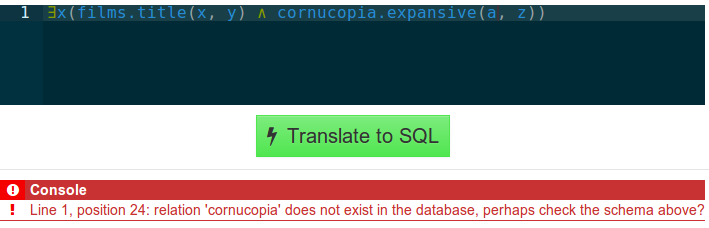
\includegraphics[width=1.0\textwidth]{images/error.png}
        \caption{A user being informed of a semantic error: the relation
          'cornucopia' does not exist in the schema.}
      \end{figure}

\section{Evaluation}
  Evaluate your deliverables e.g. performance, usability, etc.
  Summarise testing procedures + relevant testing results

  - talk about how our plan changed, how things went wrong

\section{Conclusion and Future Extensions}
  What did you learn? What might you have done differently?
  How would you build on what you have done?

  \subsection{Future Extensions}

    \subsubsection{Further Semantic Analysis}
    \todo[inline]{Can anyone think of anything beyond type checking?}

\section{Project Management - MOVE ABOVE EVALUATION}
  Planning, group organisation, breakdown + task allocation etc.

  \subsection{Planning}
    \todo[inline]{TODO Should we discuss here how everything went wrong, and
    revisions were missed entirely?}

    As we have learnt from previous projects, inside and outside the
    department, it is critical to thoroughly plan a software engineering
    exercise of this scale before beginning to implement features and write
    code. As discussed in our introduction section, we decomposed our problem
    of translating first order predicate logic to SQL into several key
    subgoals. This enabled us to outline a core feature set which we wished to
    implement and gave us a much clearer idea of how to begin tackling the
    problem.

    Moreover, we initially split the project up in to five major 'revisions'.
    Each revision added a certain amount of functionality to our project, and
    allowed us to continually build upon features already implemented. This
    incremental method of development is one of the key ideas of the Agile
    development methodology to which we adhered to throughout the project.
    \todo[inline]{TODO citation} Additionally, with each revision having a
    deadline, it gave the team a clear plan of what was to be implemented at
    what time.

    \begin{table}[H]
      \centering
      \begin{tabular}{| l | p{0.6\textwidth} | l |}
        \hline
        \textbf{Revision} & \textbf{Necessary Steps for Completion}
          & \textbf{Completion Estimate} \\
        % \multicolumn{1}{p{0.6\textwidth} |}{\textbf{}}
        \hline
        1 &
          \begin{compactitem}
            \item Set up basic web server;
            \item Set up and create a database;
            \item Create simple UI \& communicate with server;
            \item Create 5 sample Logic to SQL translations;
            \item Set up development environment.
          \end{compactitem}
          & 17/10/13 \\
        \hline
        2 &
          \begin{compactitem}
            \item UI sends predicate logic to web server;
            \item Web server parses the logic into an AST;
            \item Backend translates the AST to SQL for basic \texttt{SELECT
              FROM} queries (i.e. projection only);
            \item Create 5 more sample Logic to SQL translations.
          \end{compactitem}
          & 25/10/13 \\
        \hline
        3 &
          \begin{compactitem}
            \item Expand backend parser grammar to include more advanced use of
              SQL queries (selection \& projection);
            \item Dynamic table selection in logic - "smart" logic predicates,
              e.g. \texttt{updated(x)} vs. \texttt{customer.updated(x)};
            \item Hook into database.
          \end{compactitem}
          & 1/11/13 \\
        \hline
        4 &
          \begin{compactitem}
            \item User-defined functions;
            \item Configurable UI - database settings, and possibly changing the
              UI depending on the user's ability;
            \item Extend backend to use SQL joins.
          \end{compactitem}
          & 8/11/13 \\
        \hline
        5 &
          \begin{compactitem}
            \item Contingency time built in for bug fixes, or additional
              features/extensions depending on the project status (e.g. Semantic
              checks of logical statements before translating to SQL).
          \end{compactitem}
          & 15/11/13 \\
        \hline
      \end{tabular}
      \caption{Feature sets for each revision, as defined at the start of the
        project}
    \end{table}

  \subsection{Group Organisation}
    At the beginning of the project, as discussed previously, we outlined the
    goals and required features of our project, and split them up in to three
    rough areas - front end (handling user interactions),
    middle end (communicating between client and server), and
    then the back end (translation and database access).
    We initially split our group of six in to three teams,
    corresponding to each of the subsections of our project. Members were
    allocated to each team depending on their strengths - initially Ted and Tom
    were to complete front end work, Sam and Mitchell to do middle end, and
    Sean and Max on back end. These were just initial roles, and we found that
    throughout the project, roles could be temporarily switched around to put
    extra work in to tasks that took longer than expected.

    One of the key ways we kept our group organised was through weekly
    meetings.  During each weekly meeting, we discussed what tasks were to be
    completed that week, and spoke in detail about any concerns members had
    about the tasks that had been completed previously. We would also analyse
    the previous weeks performance, and make changes to our plan accordingly.
    This falls in line with a key principle of Agile development, where a team
    must be adapatable to change. An example of such a change is when we
    realised implementing the parser would take significantly longer than
    originally thought. This lead us to modify our feature set, reallocate
    group roles temporarily, and modify deadlines and revision subgoals.

  \subsection{Tracking}
    Once an overarching plan was agreed on, we split each major goal of each
    revision in to smaller tasks. For each of these tasks, we then allocated a
    numerical estimate of the time it would take to complete, on a scale of 1
    to 5, where 1 signified a short task and 5 signified a very time consuming
    task. The estimate of time a task would take was initially based on
    previous experience on other software engineering projects the group
    participated in, but as the project progressed, we applied knowledge of how
    prior tasks went to more accurately assign estimates.

    A typical practice in Agile development is for developers to write down
    their tasks on cards, and then place them on a physical board (known as an
    "information radiator") located in sight of all developers on the project.
    Upon this board are "swim lanes"; columns which cards belong to, and denote
    their progress (e.g. "to do", "doing" and "done"). Each task has a time
    estimate (as discussed above), and is assigned to one or more people to
    complete.  This allows every developer to know exactly what is happening at
    what time, what has to be done, and what has been completed. For our group,
    working in DoC labs and at home, this would obviously not be practical.
    Therefore, we used web-based project management software called
    Trello. This software behaves in the same way as a physical board, but is
    accessed via a web based interface which can be edited by all members of
    the project.  Additionally, each card has a hashtag which denotes which
    revision a task belongs to, or if a stricter deadline is required, a date
    for completion can be manually added.  Virtual cards are moved between each
    swim lane as the task progresses. The group found this tool indispensible
    for communication and keeping on track with the project.

    \todo[inline]{TODO Citations for the above agile stuff}

    \begin{figure}[h!]
      \centering
      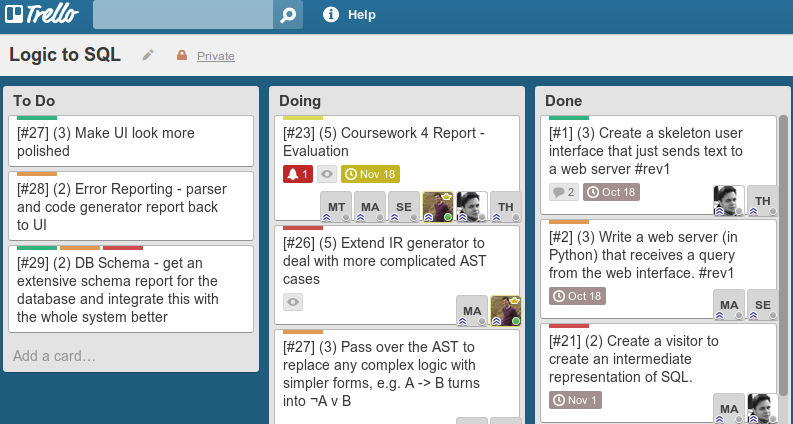
\includegraphics[width=0.9\textwidth]{images/trello.png}
      \caption{A screenshot of our Trello board toward the end of our project.}
    \end{figure}

  \subsection{Version Control and Automated Testing}
  -- "You shall not pass" commit msg. Definitely needs the picture.

    -- Trello, Git integration

    -- Burndown chart

    -- nosetests

    -- CI server

\section{Bibliography}
  \printbibliography

  --TODO Agree on referencing practice. The library recommends Harvard. --

  https://workspace.imperial.ac.uk/library/Public/Harvard\_referencing.pdf

\appendix
\section{Appendix}
  The appendix is optional, and does not count towards the 35 pages. It may
  contain thing like: User guide, installation instructions; more extensive
  design, testing, statistics etc.

  \subsection{Installation Guide}

  - Sean will do this (I have a list of dependencies ready)

  - need to mention not posibul 2 instal the earlangs on the gentoo pls

  \subsection{UML Diagram}

  - Look online to see if this can be generated by any tools.

  - Or make a reduced one, just showing main components of the project e.g.
  parser, sql generator, semantic analyser, etc

  \subsection{'filmdb' Schema}

  \subsection{Design Diagrams}

  - things like sean's bullshit rough drawings from Chatley reports

  \subsection{Statistics}

  - This is just the performance metric, profiling etc diagrams from 
  Chatley coursework 4.

%\section{Anandha waffle from his site - delete once finished report}
%  Final Report ? due: 13th Jan 2014, at 16:00 (both Electronic and Hardcopy)
%
%  Contents for Final Report: The project report should not be longer than 35
%  pages (recommended length is around 30 pages), and might be organised
%  according to the following structure: see above sections
%
%  Make sure that the final report presents a coherent story. Ask advice from
%  your supervisor. You might also draw inspiration from the instructions about
%  writing up your individual project.
%
%  Bear in mind, that most of the project assessors will not have followed the
%  project throughout and will only have a short time to listen to a
%  presentation or see a demonstration. For this reason they will rely heavily
%  on the report to judge the project.
%
%  The report should be submitted to SGO in form of a hard copy, as well as
%  electronically through CATE. i.e. report.pdf. 
%
%  ------------------------
%
%  Assessment
%  Will be updated soon.
%
%  Group project
%  The group project assessment is undertaken by each group's supervisor, and
%  moderated by a larger group of assessors, who will attend your presentation,
%  and/or read your final report. The assessment is based on:
%
%      Executive Summary, 5
%      Presentation, 10
%      Group Collaboration and Management, 20
%      Report, 30
%      Technical Achievement, 35
%
%  The group project (along with the Software Engineering course) is worth 440
%  Marks for both the MEng and BEng students.
%  Overall assessment
%  The overall assessment is the sum of the group project component and the
%  Software Engineering Course in an 80:20 split.
%
\end{document}
